\section*{Áttekintés}

A mérés során vizsgált szuperheterodin elvű adólánc blokkvázlata a \ref{fig:ado}. ábrán látható. Az alapsávi jelet egy BPSK, illetve OOK modulációra képes modulátorral állítjuk elő, amit egy $\SI{16}{MHz}$-es vivőre kerül. Ezt szűrés után egy gyűrűs DBM keverő segítségével középfrekvenciára, $\SI{434}{MHz}$-re keverjük fel, a keveréshez $\SI{450}{MHz}$-es lokál oszcillátort (LO) használunk. KF szinten szűrés után felkeverjük a jelet $\SI{2.4}{GHz}$-es RF sávra egy PLL-es keverő segítségével. KF és RF fokozaton opcionálisan erősítőt is hozzáadhatunk az adólánchoz, ettől a mérés során eltekintettünk.

\begin{figure}[H]
	\centering
	\includegraphics[width=0.7\textwidth,keepaspectratio]{kepek/ado.PNG}
	\caption{Az adólánc blokkvázlata}
	\label{fig:ado}
\end{figure}

A vevőlánc a \ref{fig:vevo}. ábrán látható, az antenna helyett jelgenerátort használtunk, amin azonban csak modulálatlan $\SI{16}{MHz}$-es alapsávi vivőt használtunk. Rádiófrekvenciáról középfrekvenciára, illetve középfrekvenciáról alapsávra ugyanolyan keverőket, illetve sávszűrőket használtunk, mint az adó esetében. Ellenben az erősítőket ebben az esetben nem hagytuk ki, ugyanis a lekeverések és a szűrések során a hasznos jelünk eltűnne a zajban.

\begin{figure}[H]
	\centering
	\includegraphics[width=0.7\textwidth,keepaspectratio]{kepek/vevo.PNG}
	\caption{A vevőlánc blokkvázlata}
	\label{fig:vevo}
\end{figure}

\section*{Adólánc}

A modulátor mindkét üzemállapotában jelentős felharmonikus tartalmat bocsát ki, a kimenetén a $\SI{16}{MHz}$-es alapsávú vivő felharmonikusai figyelhetőek meg. Amint a \ref{fig:modulator}. ábrán a fekete maxhold görbén látható, nem minden felharmonikus jelenik meg, például a 3., ami $\SI{48}{MHz}$-nél lenne, egyik modulációnál sem látható.

\begin{figure}[H]
	\centering
	\begin{subfigure}[b]{0.49\textwidth}
		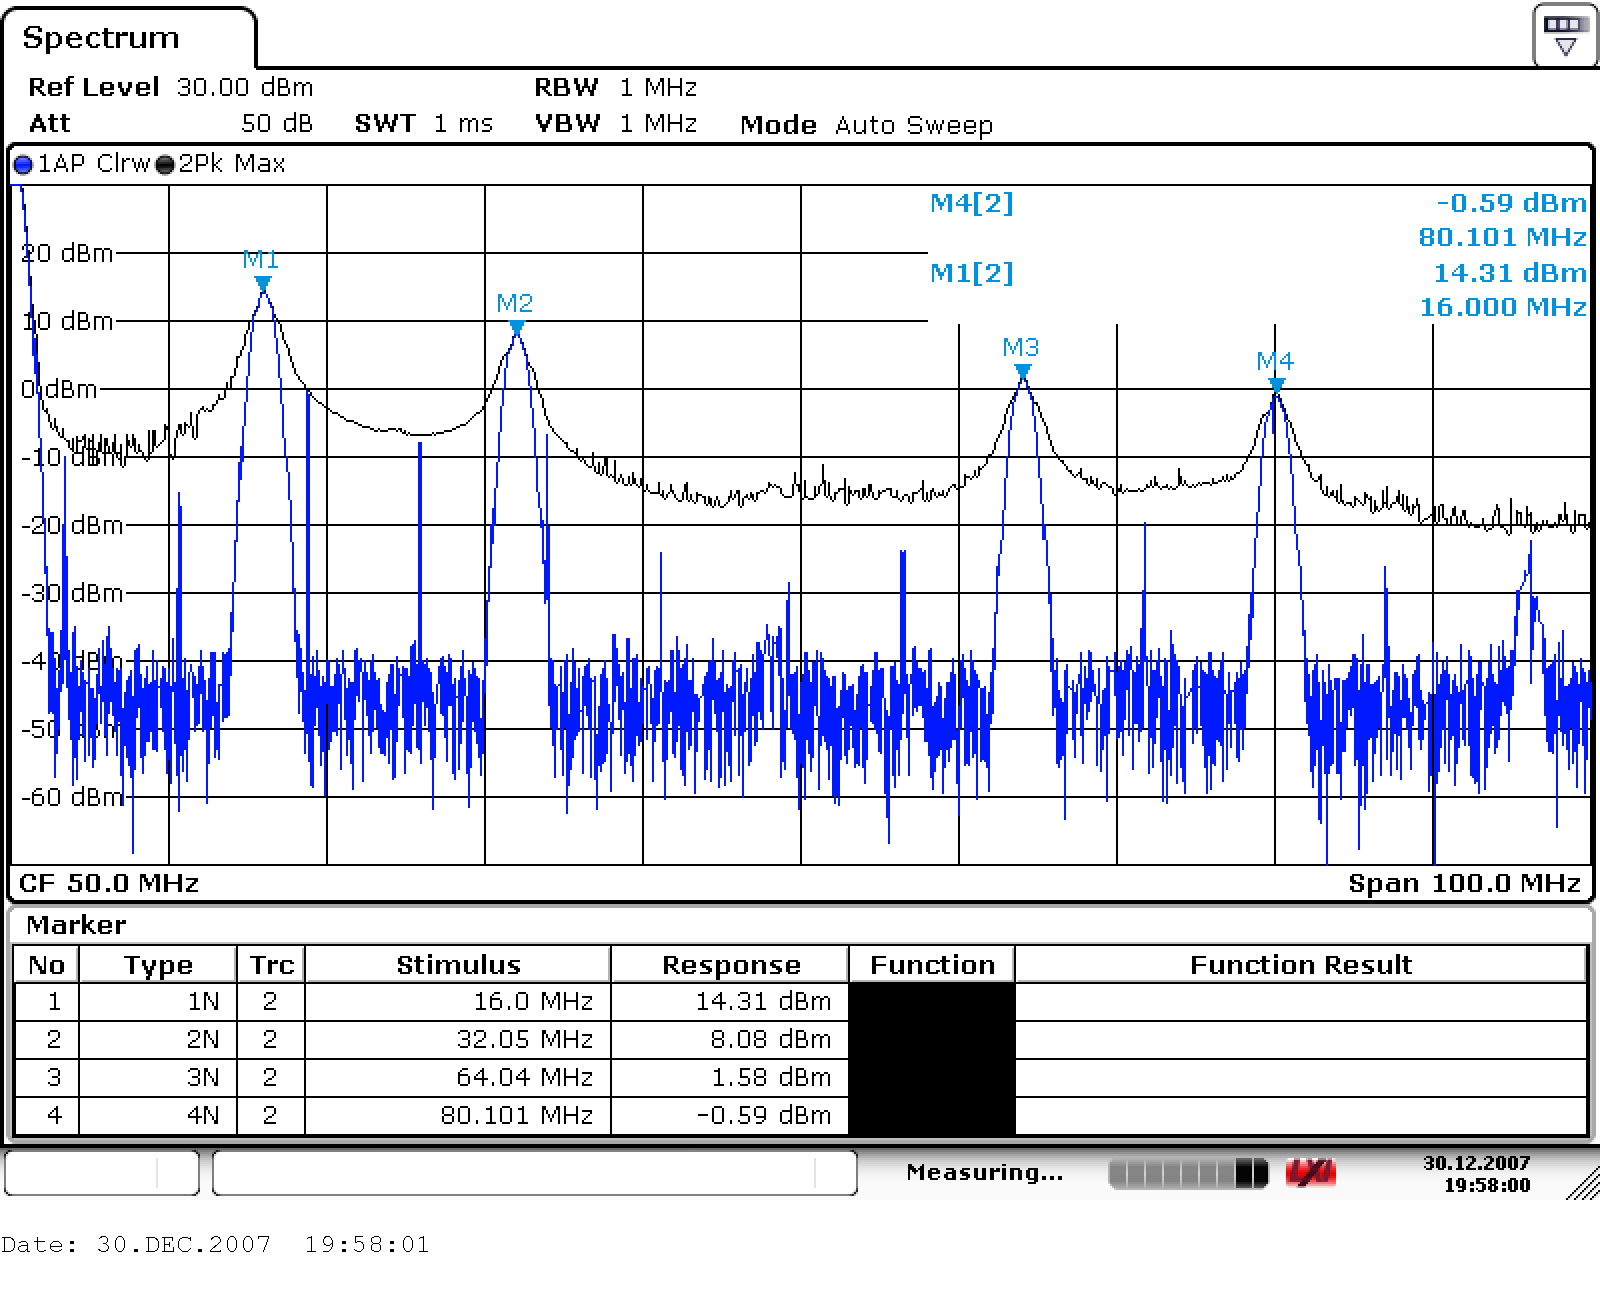
\includegraphics[width=\textwidth,keepaspectratio]{kepek/A_csop_004.PNG}
		\caption{BPSK moduláció}
		\label{fig:modulator_bpsk}
	\end{subfigure}
	\begin{subfigure}[b]{0.49\textwidth}
		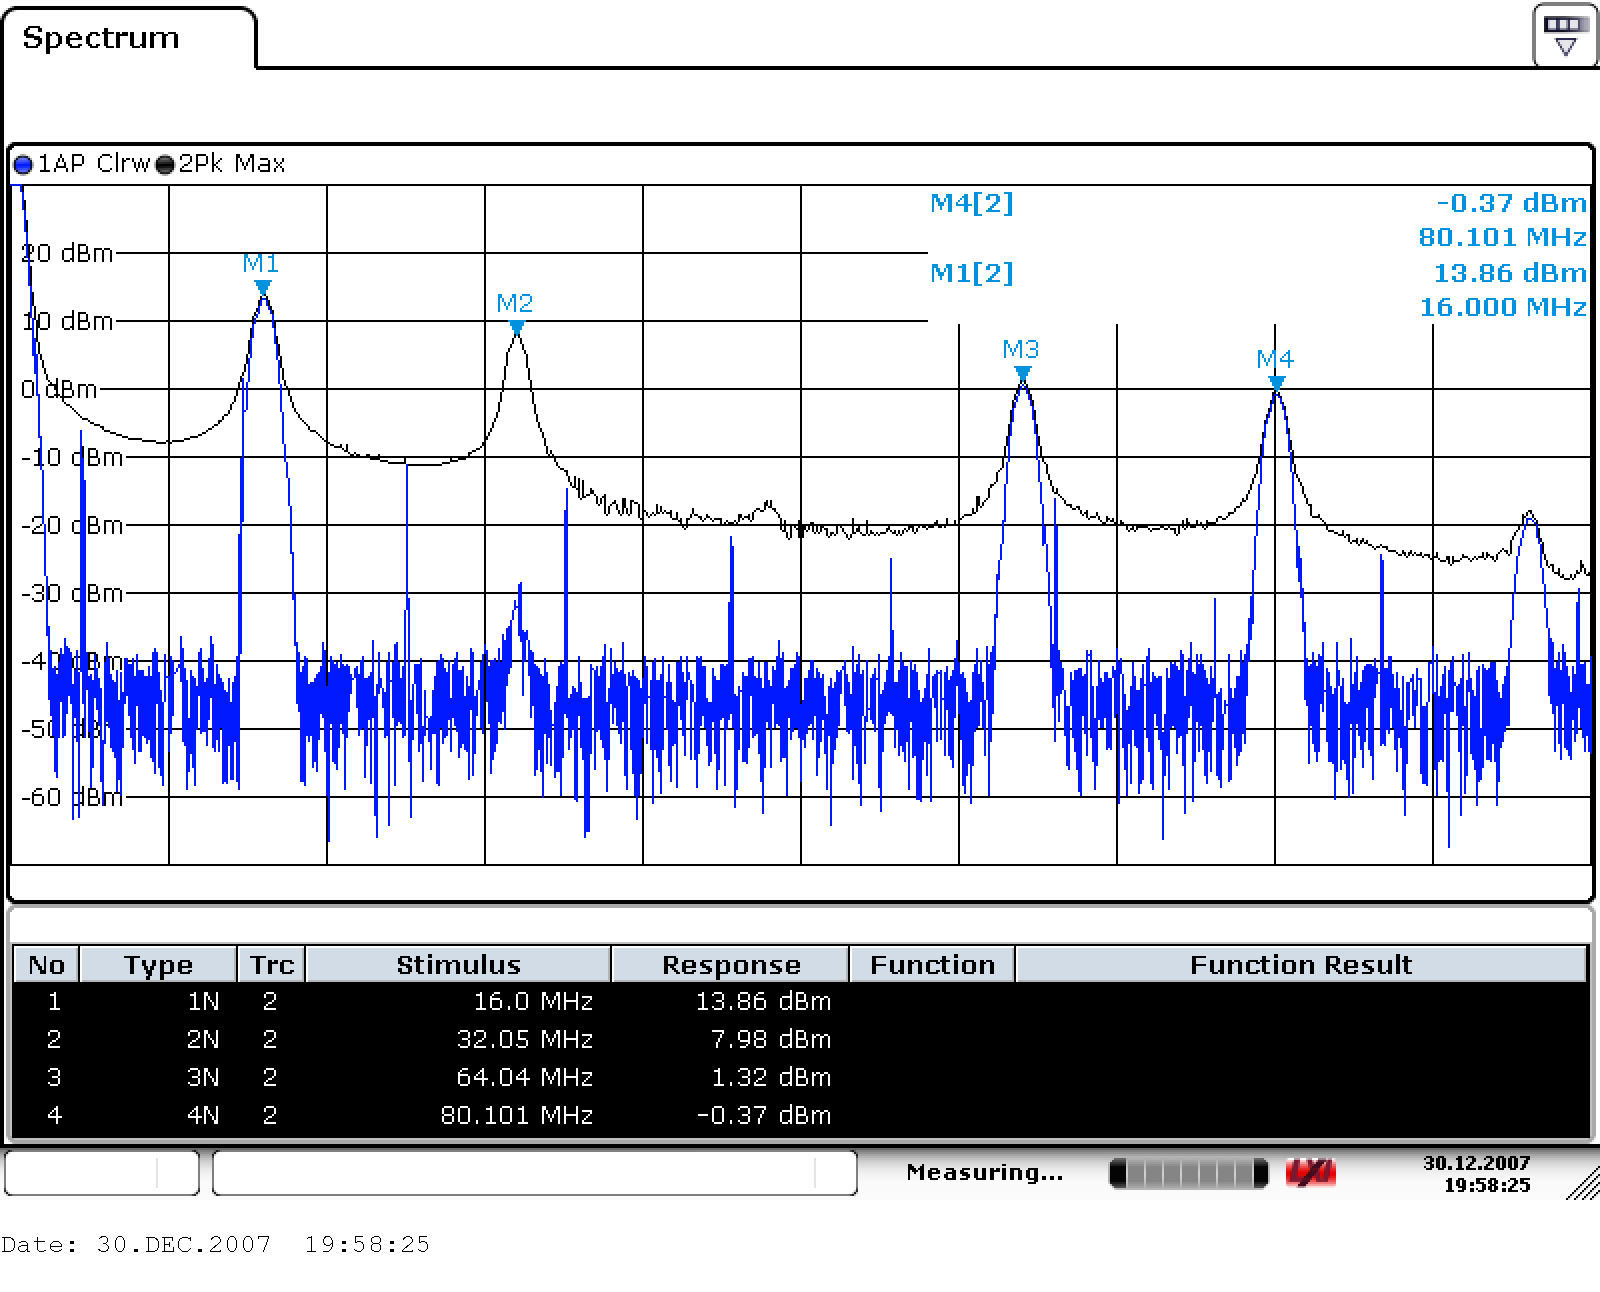
\includegraphics[width=\textwidth,keepaspectratio]{kepek/A_csop_005.PNG}
		\caption{OOK moduláció}
		\label{fig:modulator_ook}
	\end{subfigure}
	\caption{Modulátor szűrés előtti kimenete a két üzemállapotban.}
	\label{fig:modulator}
\end{figure}

Az első, második, negyedik és ötödik harmonikus frekvenciáját és a spektrumanalizátorral mért szintjét az alábbi táblázat foglalja össze mindkét modulációra.
%
\begin{table}[H]
	\centering
	\caption{Harmonikusok frekvenciája és $\si{dBm}$-ben mért szintjei BPSK és OOK moduláció esetén.}
	\label{table:kondi_geometria}
	\begin{tabular}{ | c | c | c |} 
		\hline
		\textbf{Frekvencia}&\textbf{BPSK}&\textbf{OOK}\\
		\hline
		$\SI{16}{MHz}$&$\SI{14.31}{dBm}$&$\SI{13.86}{dBm}$\\
		\hline
		$\SI{32}{MHz}$&$\SI{8.08}{dBm}$&$\SI{7.98}{dBm}$\\
		\hline
		$\SI{64}{MHz}$&$\SI{1.58}{dBm}$&$\SI{1.32}{dBm}$\\
		\hline
		$\SI{80}{MHz}$&$\SI{-0.59}{dBm}$&$\SI{-0.37}{dBm}$\\
		\hline
	\end{tabular}
\end{table}

A jelalakot időben is megfigyelhetjük, ha oszcilloszkópra vezetjük a modulátor kimenetét, ezt mutatja a \ref{fig:modulator_scope}. ábra, a BPSK esetében a fázisváltást látjuk, az OOK-nál bedig a "0/1" átmenetet. A jelalakok láthatóan nem szinuszosak, a felharmonikusok torzítása ellen szűrés szükséges.

\begin{figure}[H]
	\centering
	\begin{subfigure}[b]{0.49\textwidth}
		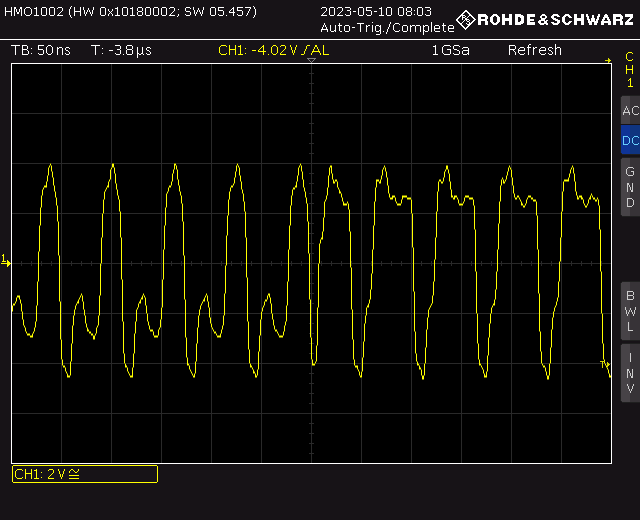
\includegraphics[width=\textwidth,keepaspectratio]{kepek/SCOPE16.PNG}
		\caption{BPSK}
		\label{fig:modulator_bpsk_scope}
	\end{subfigure}
	\begin{subfigure}[b]{0.49\textwidth}
		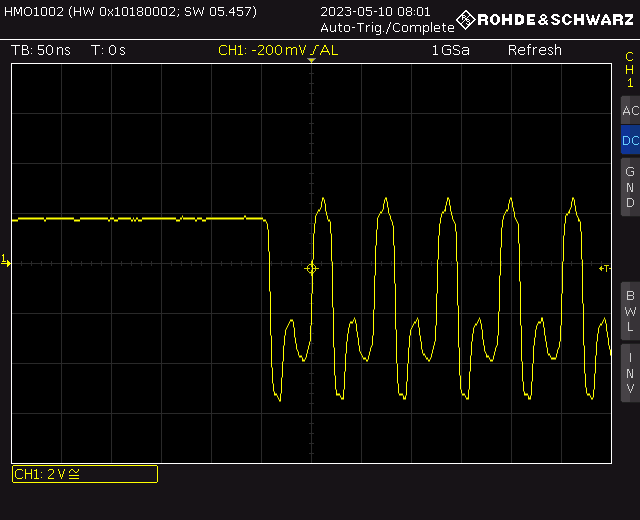
\includegraphics[width=\textwidth,keepaspectratio]{kepek/SCOPE15.PNG}
		\caption{OOK}
		\label{fig:modulator_ook_scope}
	\end{subfigure}
	\caption{Modulátor kimenete oszcilloszkópon.}
	\label{fig:modulator_scope}
\end{figure}

A modulátor kimenetére egy $\SI{16}{MHz}$-es sávszűrőt helyeztünk el, a \ref{fig:modulator_szures}. ábrán bal oldalt a szűretlen maxhold (fekete) és a már szűrt folytonosan mintavételezett jelet (kék) láthatjuk, jobb oldalt pedig már a szűrés utáni maxhold érték szerepel.

\begin{figure}[H]
	\centering
	\begin{subfigure}[b]{0.49\textwidth}
		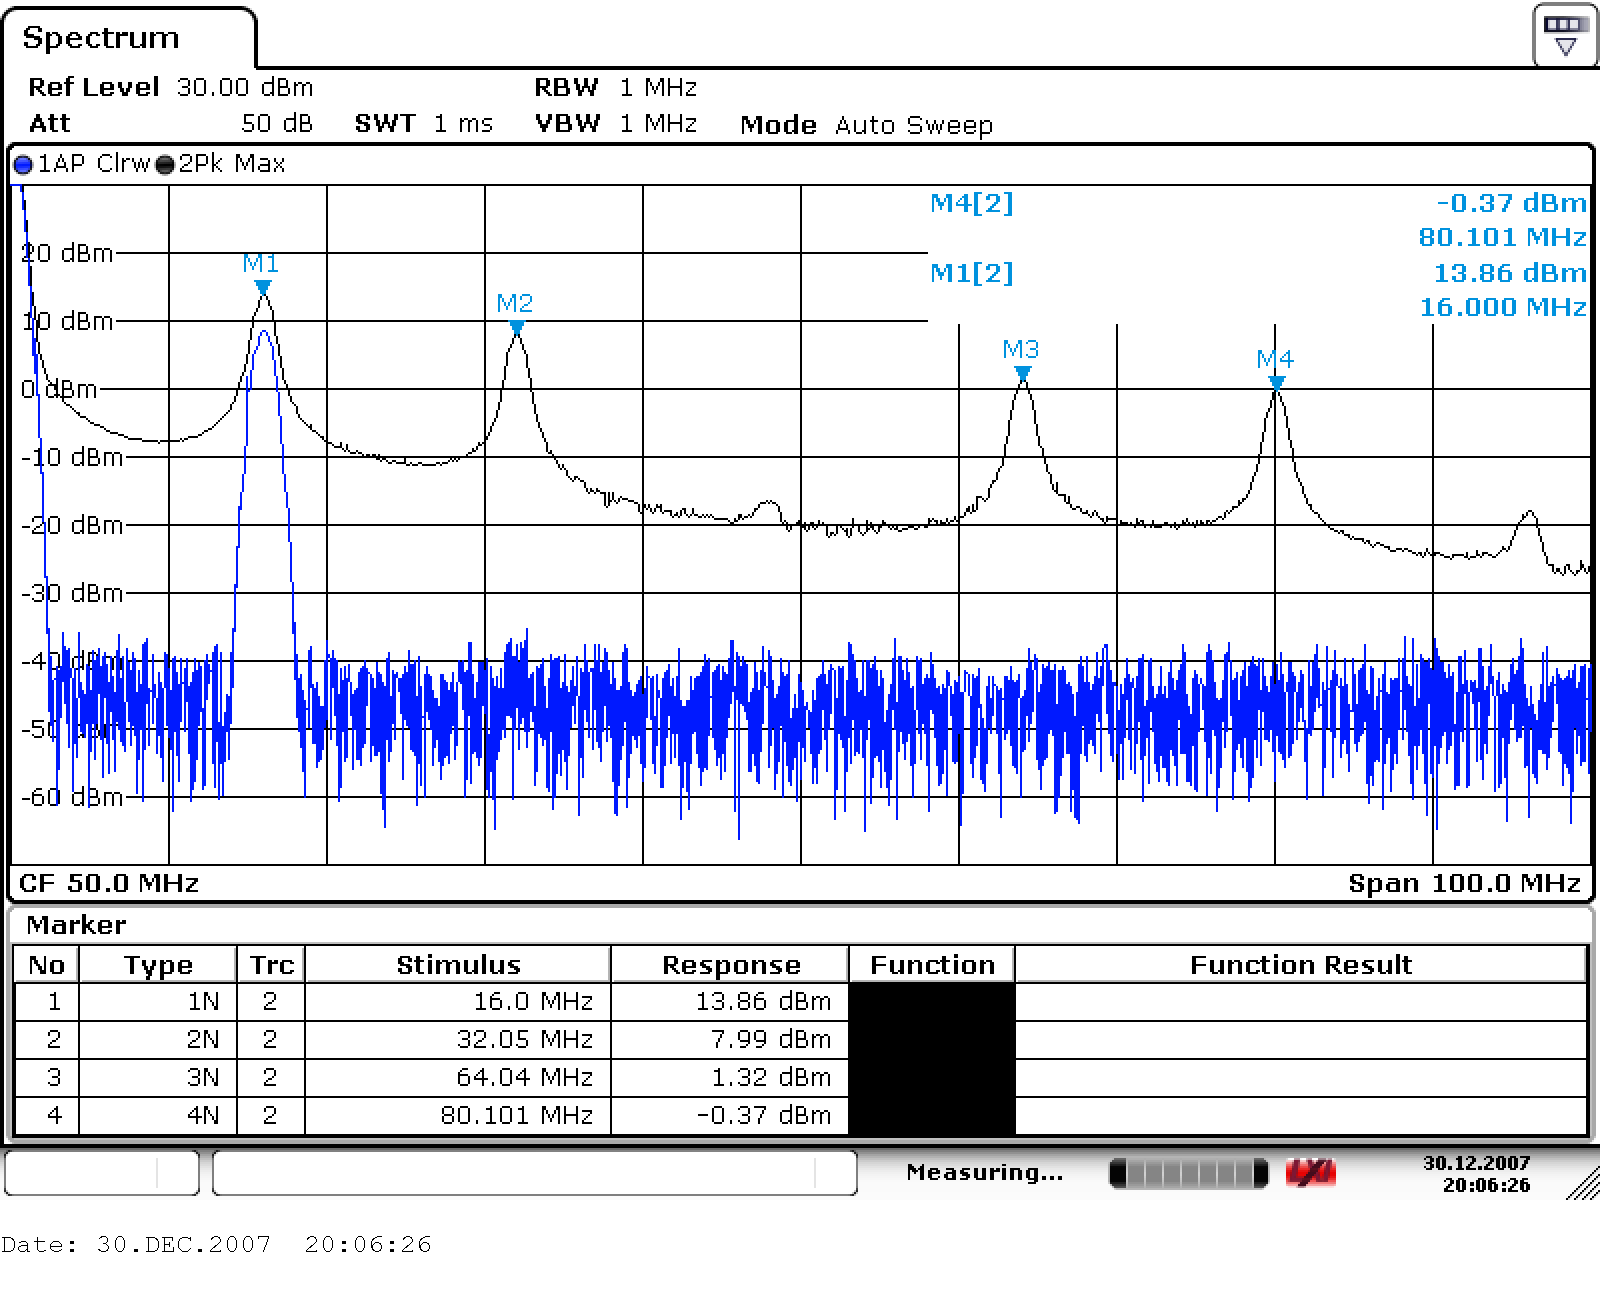
\includegraphics[width=\textwidth,keepaspectratio]{kepek/A_csop_006.PNG}
		\caption{Előtte-utána}
		\label{fig:modulator_szures_elotte}
	\end{subfigure}
	\begin{subfigure}[b]{0.49\textwidth}
		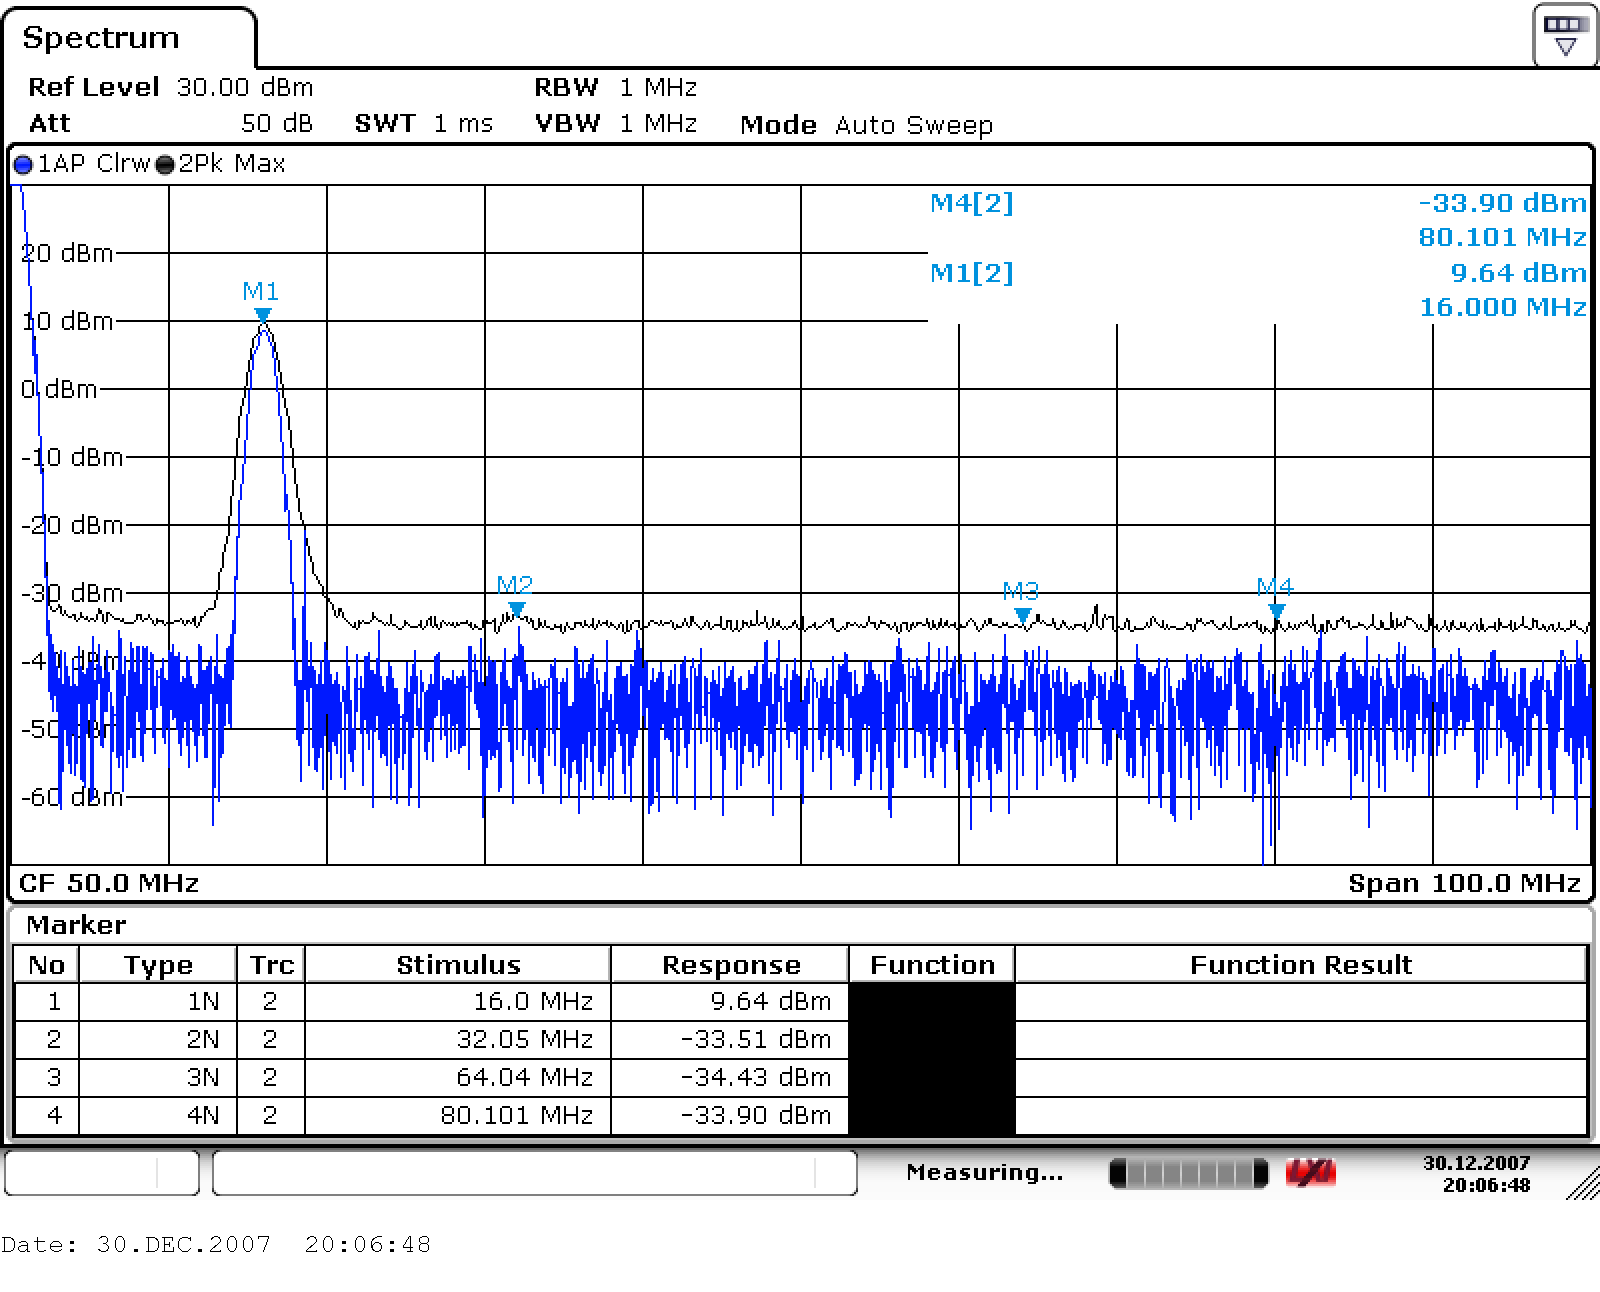
\includegraphics[width=\textwidth,keepaspectratio]{kepek/A_csop_007.PNG}
		\caption{Utána}
		\label{fig:modulator_szures_utana}
	\end{subfigure}
	\caption{Kimeneti spektrum alapsávi szűrés után.}
	\label{fig:modulator_szures}
\end{figure}

A szűretlen esethez hasonlóan megnéztük a két modulációtípust oszcilloszkópon, a \ref{fig:modulator_szures_scope}. ábrán a BPSK-nál a fázisváltás, az OOK-nál az "on/off" átmenet látható. A \ref{fig:modulator_scope}. ábrán látható felharmonikus torzítással ellentétben itt tisztán szinuszos jel mérhető.

\begin{figure}[H]
	\centering
	\begin{subfigure}[b]{0.49\textwidth}
		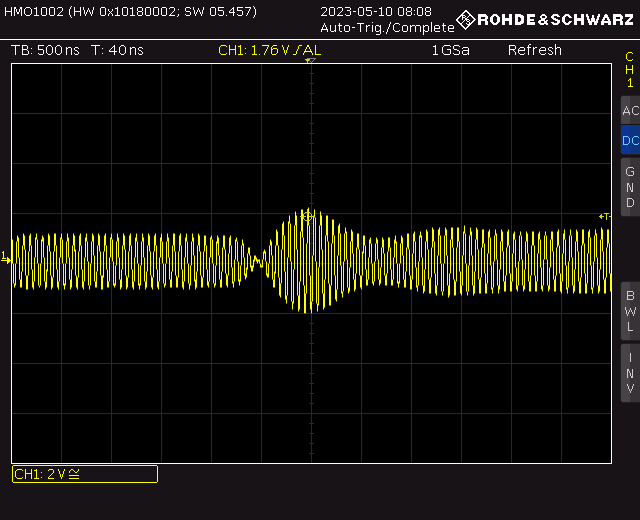
\includegraphics[width=\textwidth,keepaspectratio]{kepek/SCOPE17.PNG}
		\caption{BPSK}
		\label{fig:modulator_bpsk_scope}
	\end{subfigure}
	\begin{subfigure}[b]{0.49\textwidth}
		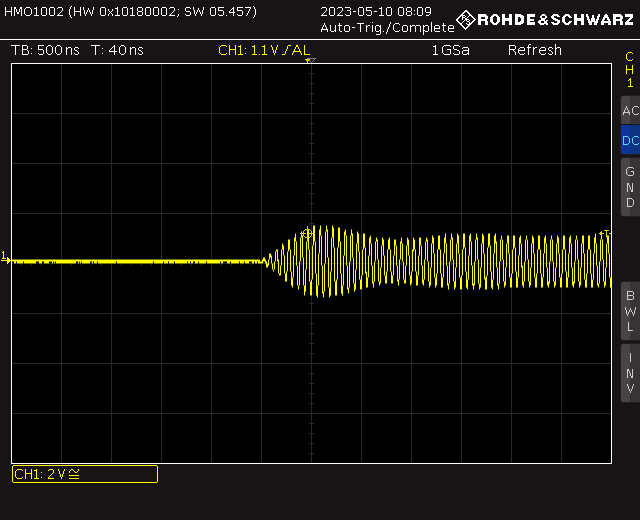
\includegraphics[width=\textwidth,keepaspectratio]{kepek/SCOPE18.PNG}
		\caption{OOK}
		\label{fig:modulator_ook_scope}
	\end{subfigure}
	\caption{Modulátor kimenete szűrés után oszcilloszkópon.}
	\label{fig:modulator_szures_scope}
\end{figure}

Középfrekvenciára, a $\SI{16}{MHz}$-ről $\SI{434}{MHz}$-re való felkeveréshez egy $\SI{450}{MHz}$-es LO-t használtuk, ennek a spektrumát mutatja a \ref{fig:LO_450}. ábra.

\begin{figure}[H]
	\centering
	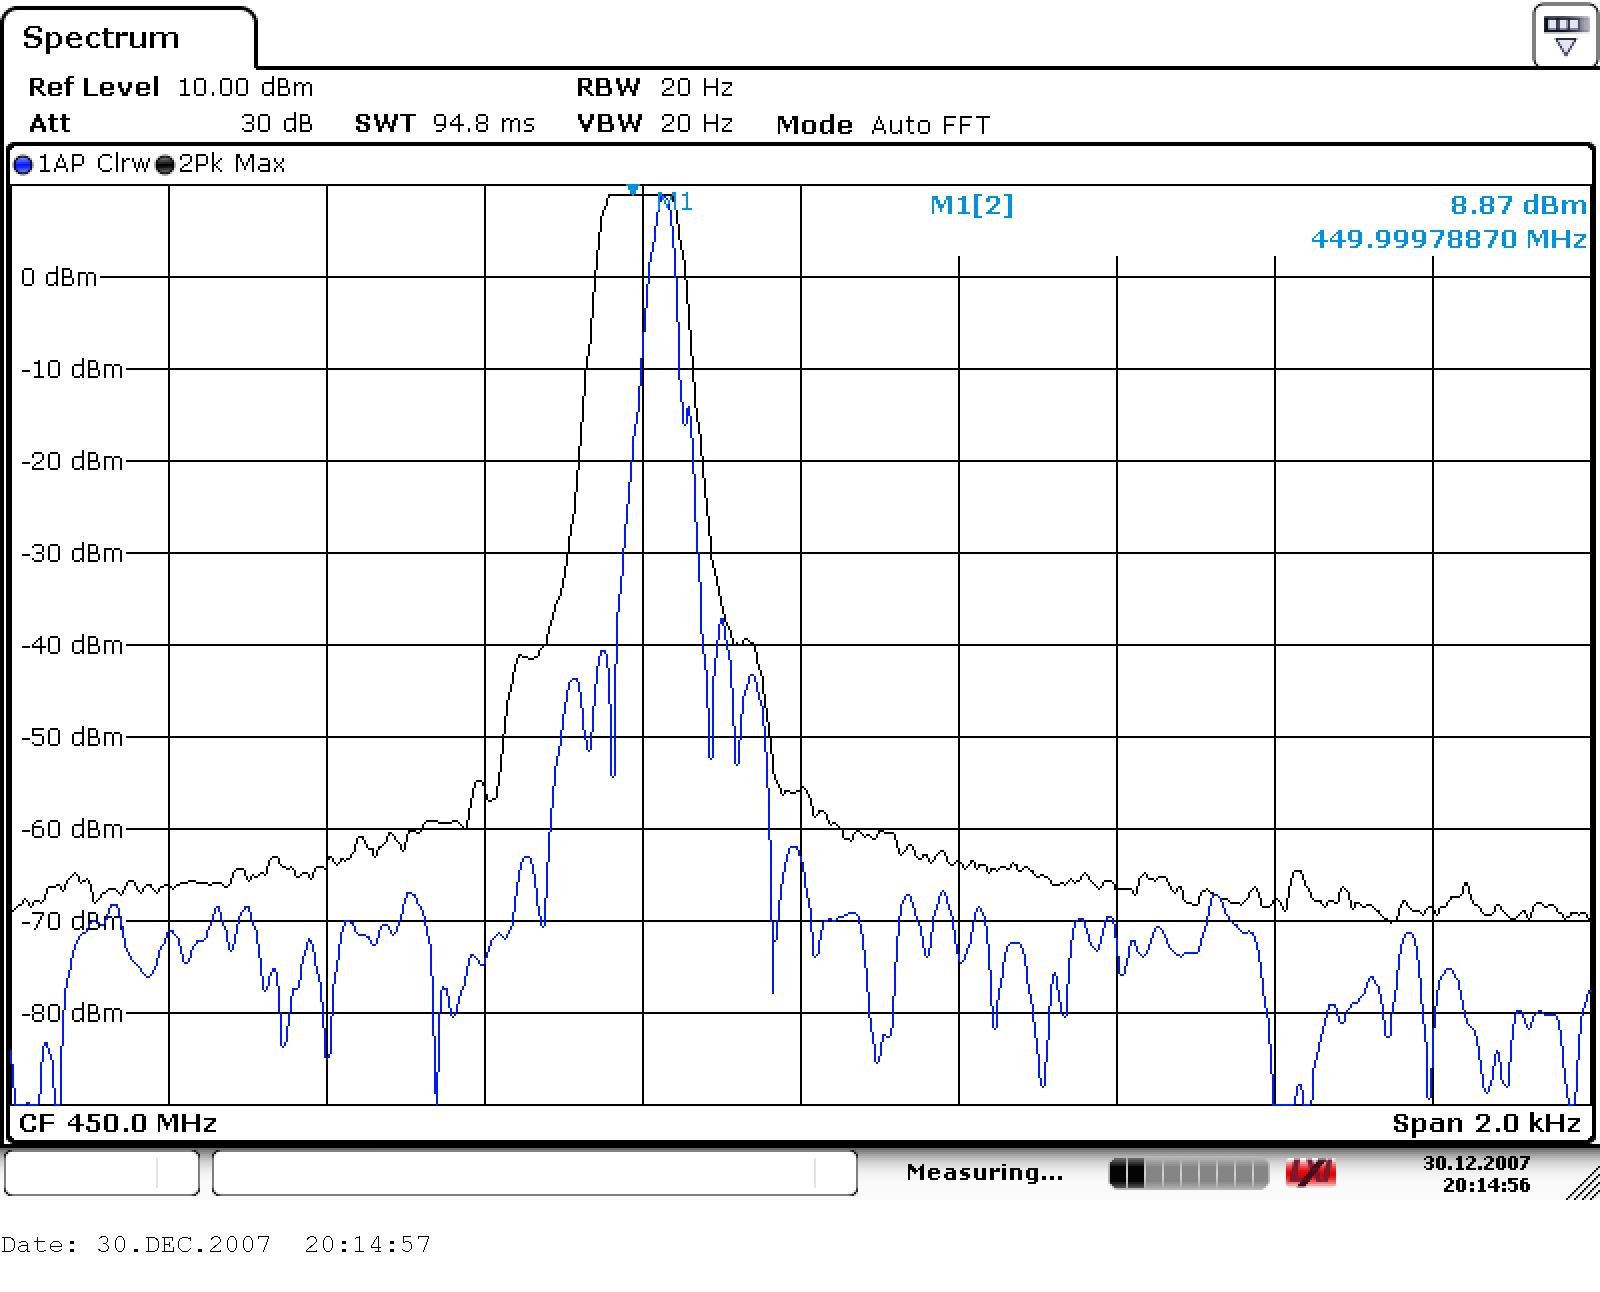
\includegraphics[width=0.5\textwidth,keepaspectratio]{kepek/A_csop_009.PNG}
	\caption{$\SI{450}{MHz}$-es LO spektruma.}
	\label{fig:LO_450}
\end{figure}

Alapszabály, miszerint keverés után szűrni kell, a keveredési termékeket egy $\SI{434}{MHz}$-es sávközepű sávszűrővel nyomjuk el. A szűrés előtti és utáni középfrekvenciás spektrumot a \ref{fig:KF}. ábra mutatja, a hasznos jel közel $\SI{1.7}{dB}$-t, míg a tükörfrekvenciás komponensek $\SI{450}{MHz}$-en és $\SI{466}{MHz}$-en $\SI{40}{dB}$-lel, illetve $\SI{44.5}{dB}$-lel csillapodtak.

\begin{figure}[H]
	\centering
	\begin{subfigure}[b]{0.49\textwidth}
		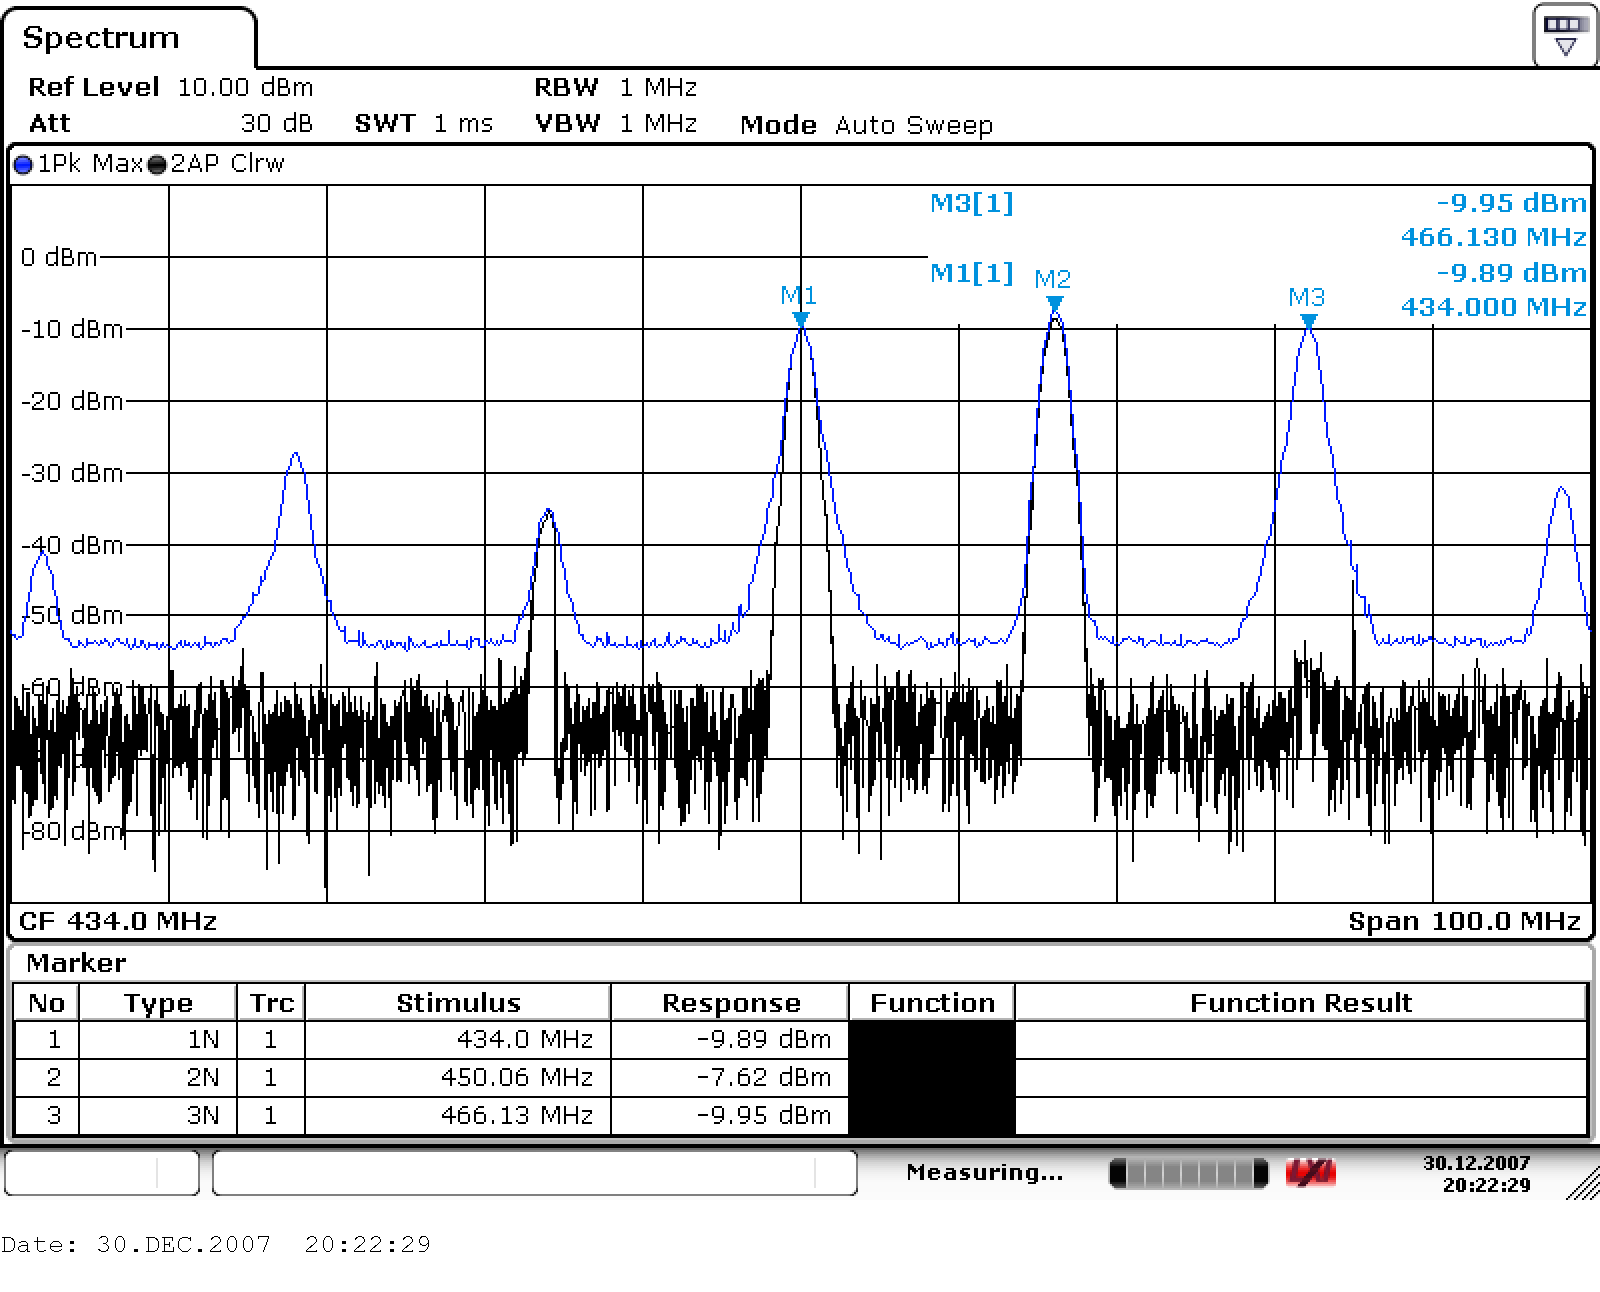
\includegraphics[width=\textwidth,keepaspectratio]{kepek/A_csop_010.PNG}
		\caption{Szűrés előtt}
		\label{fig:KF_elotte}
	\end{subfigure}
	\begin{subfigure}[b]{0.49\textwidth}
		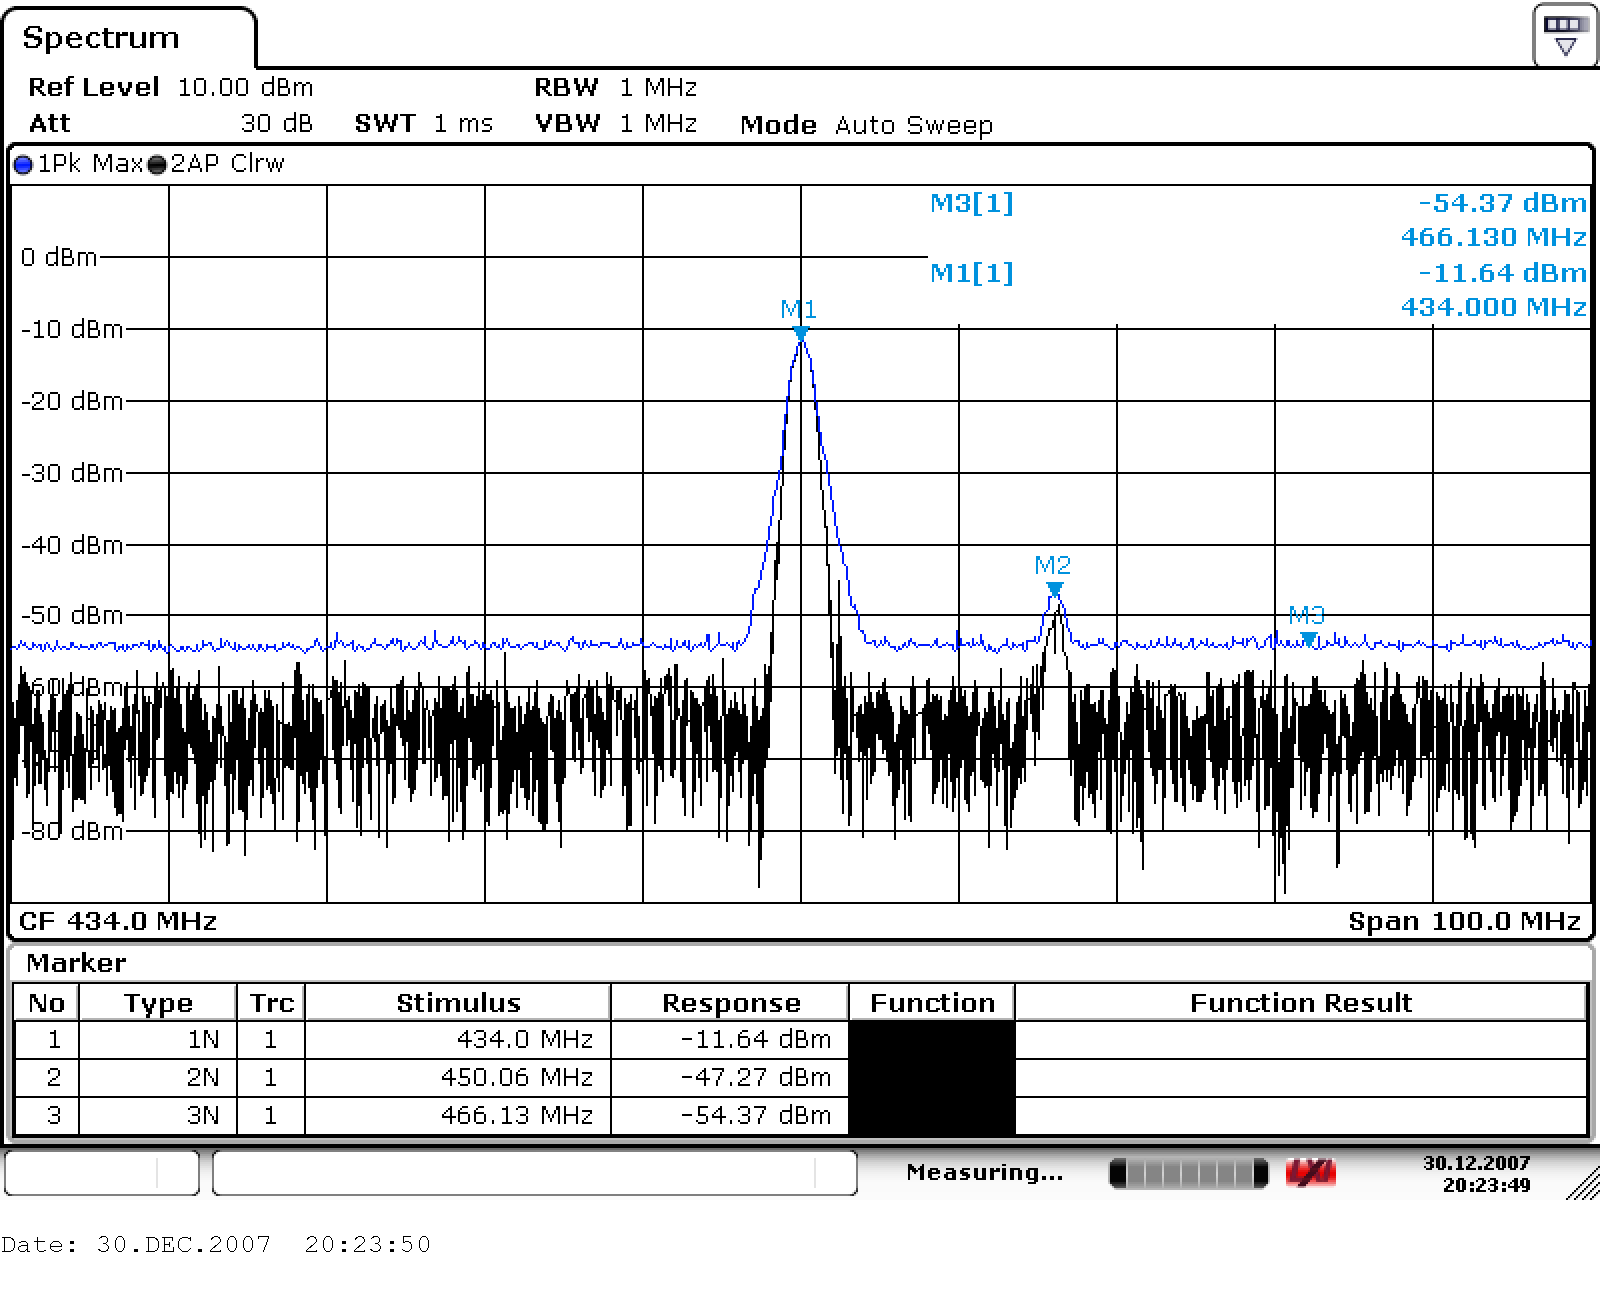
\includegraphics[width=\textwidth,keepaspectratio]{kepek/A_csop_011.PNG}
		\caption{Szűrés után}
		\label{fig:KF_utana}
	\end{subfigure}
	\caption{Középfrekvenciás spektrum szűrés előtt, illetve szűrés után.}
	\label{fig:KF}
\end{figure}

Rádiófrekvenciás fokozatra, a $\SI{434}{MHz}$-ről $\SI{2.4}{GHz}$-re keveréshez egy $\SI{1.966}{GHz}$-es LO szükséges, amit egy fáziszárt hurok, egy PLL áramkör valósít meg. Ennek a spektrumát mutatja a \ref{fig:PLL}. ábra, jobb oldalon kicsi, $\SI{2}{MHz}$-es span mellett vizsgáltuk meg, ahol megfigyelhető a szoknyásodás.

\begin{figure}[H]
	\centering
	\begin{subfigure}[b]{0.49\textwidth}
		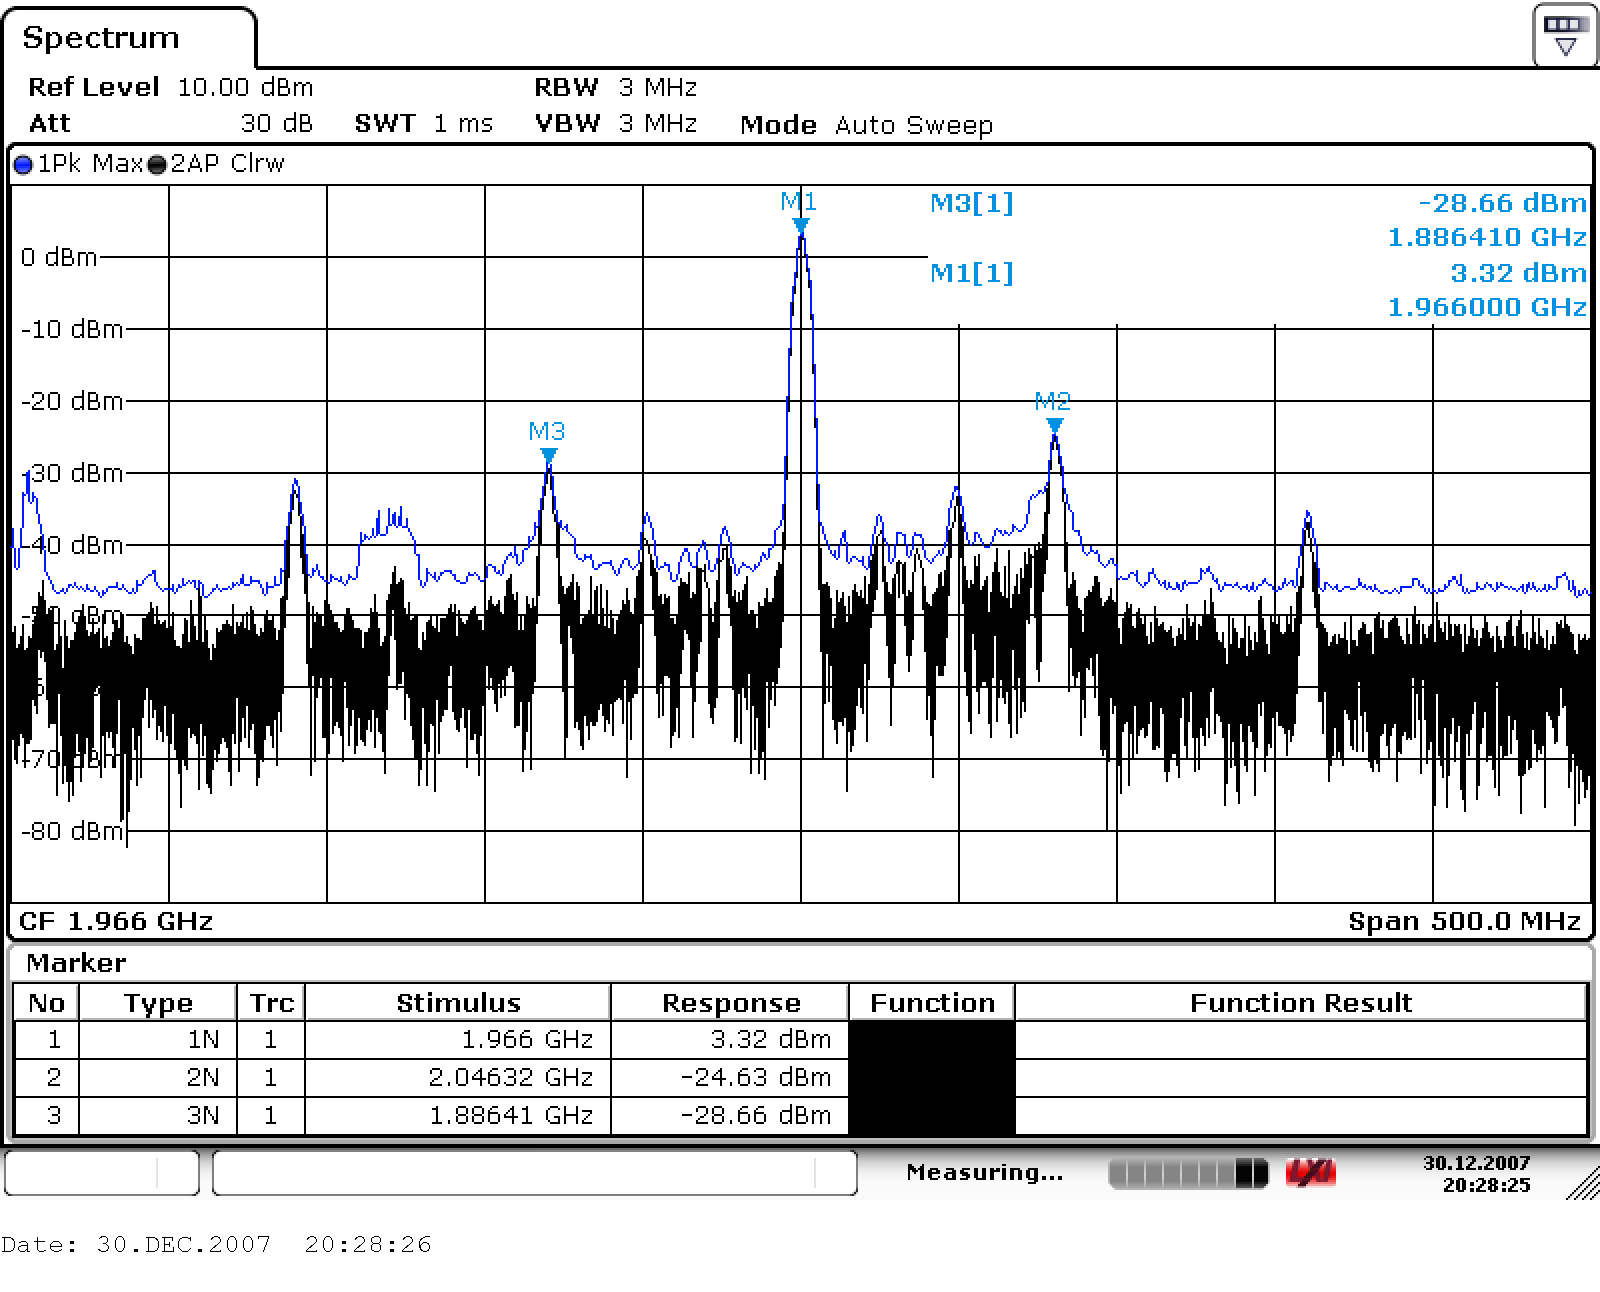
\includegraphics[width=\textwidth,keepaspectratio]{kepek/A_csop_012.PNG}
		\caption{Span = $\SI{500}{MHz}$}
		\label{fig:PLL_span500}
	\end{subfigure}
	\begin{subfigure}[b]{0.49\textwidth}
		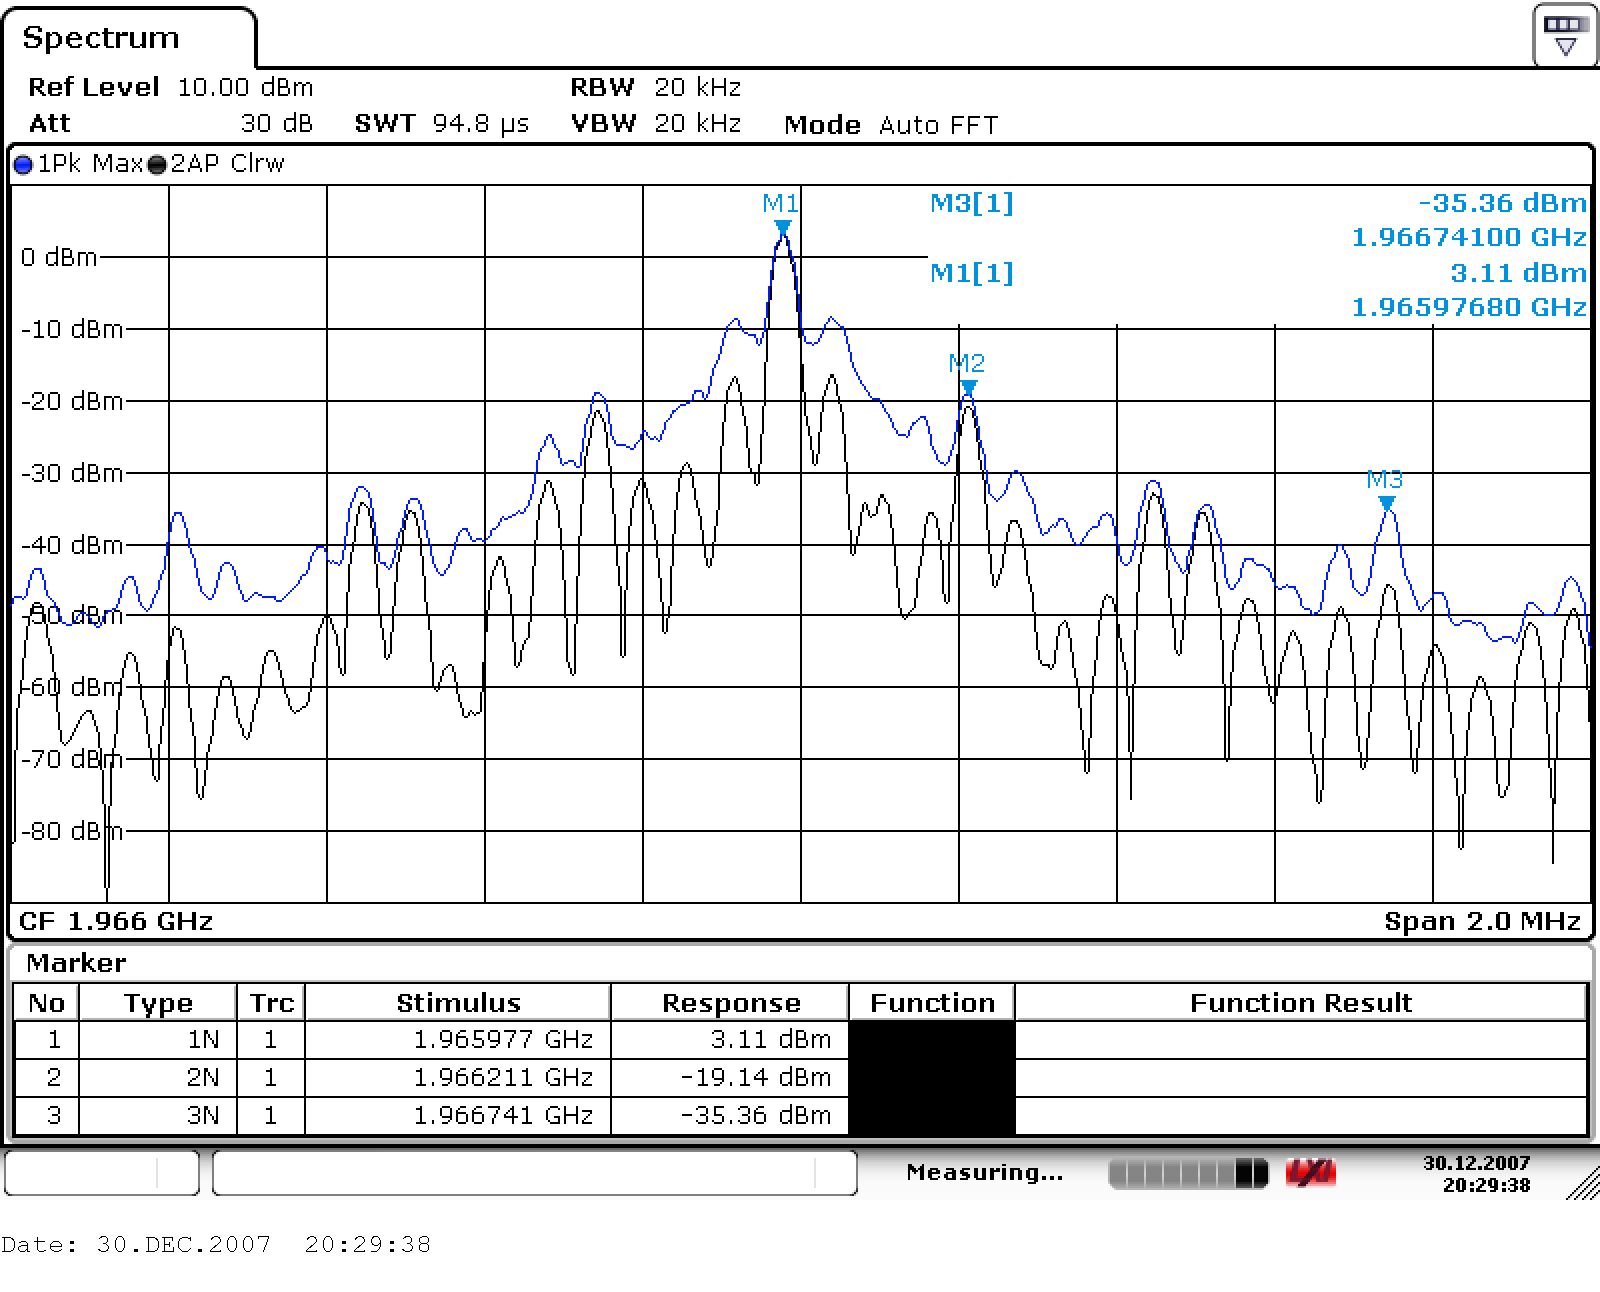
\includegraphics[width=\textwidth,keepaspectratio]{kepek/A_csop_013.PNG}
		\caption{Span = $\SI{2}{MHz}$}
		\label{fig:PLL_span2}
	\end{subfigure}
	\caption{A PLL áramkör kimeneti spketruma.}
	\label{fig:PLL}
\end{figure}

RF keverés után ismét megjelennek keveredési termékek, egy $\SI{2.4}{GHz}$-es sávszűrővel ezek kiszűrhetőek, amint azt a \ref{fig:RF}. ábra mutatja. A hasznos jel $\SI{5.1}{dB}$-lel, a zajkomponensek pedig $\SI{33}{dB}$-lel, illetve $\SI{26.4}{dB}$-lel csillapodtak.

\begin{figure}[H]
	\centering
	\begin{subfigure}[b]{0.49\textwidth}
		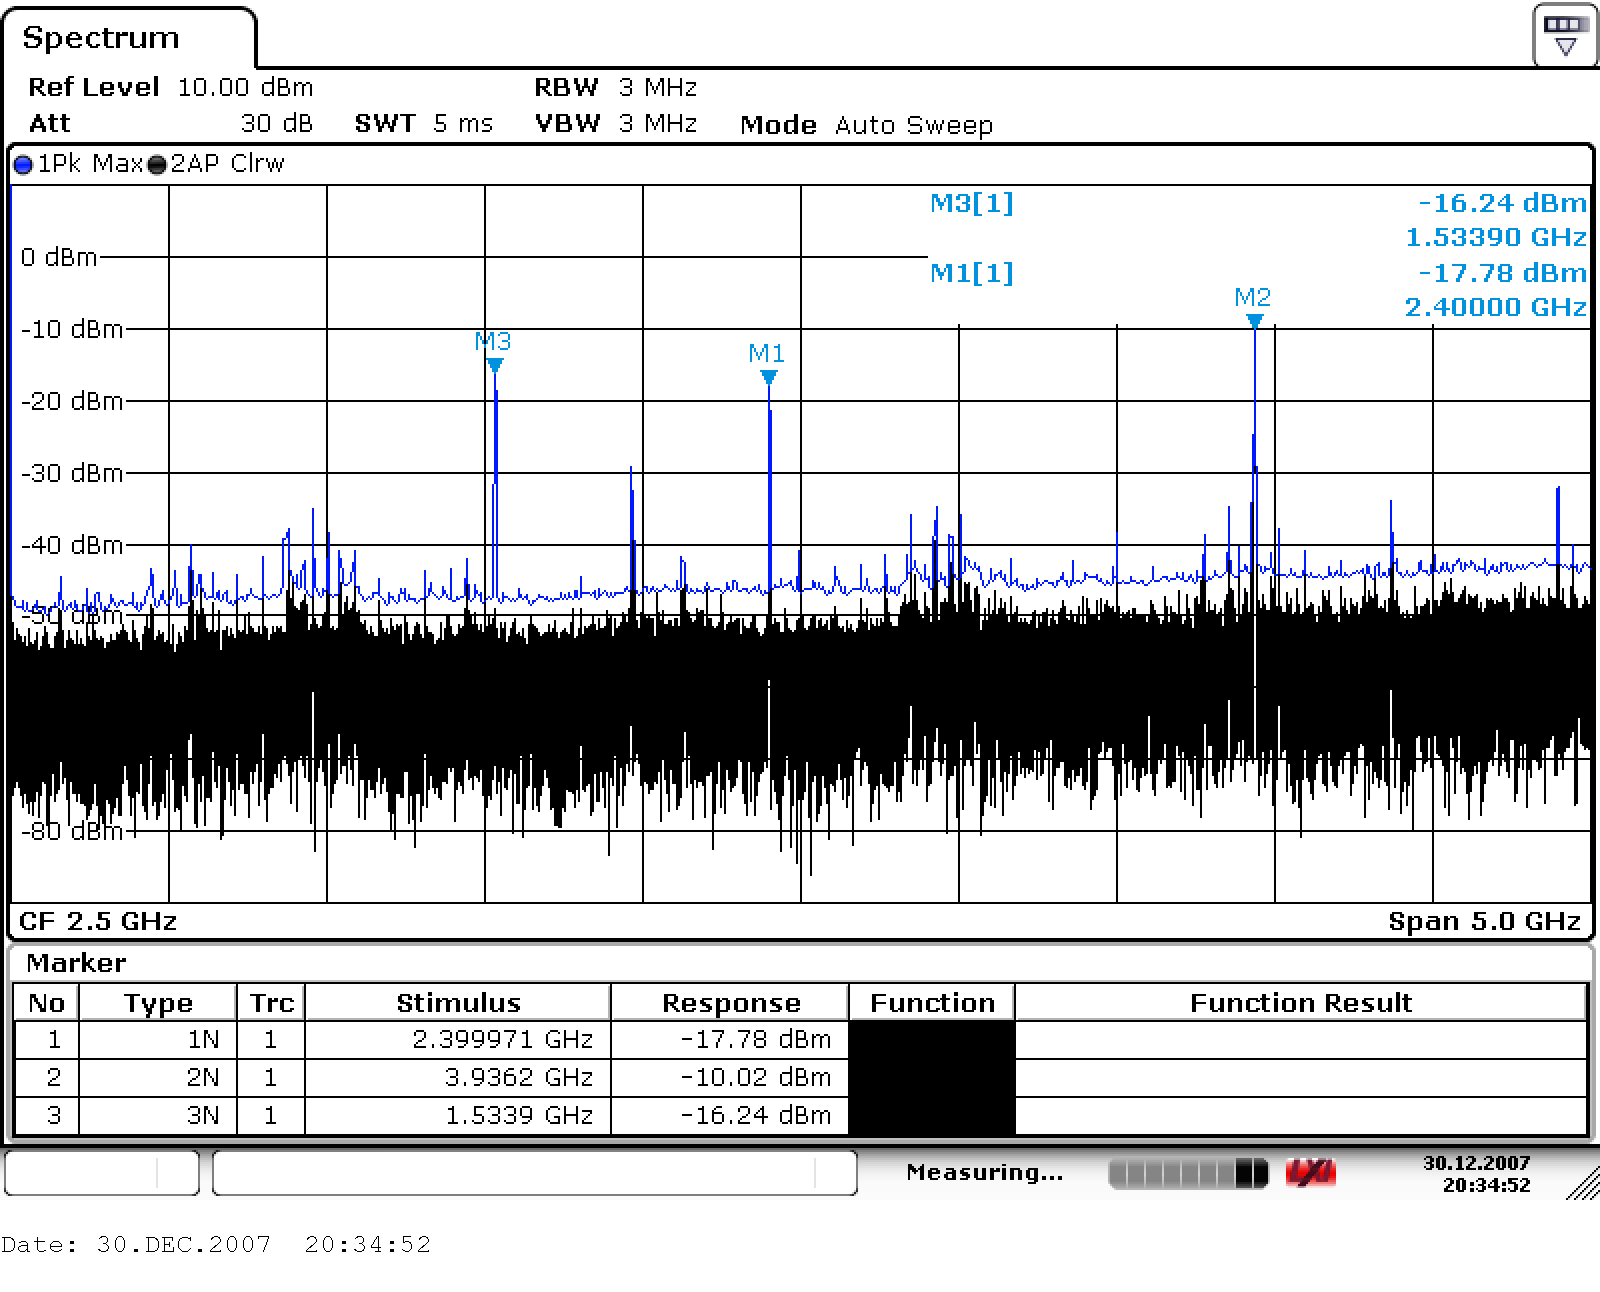
\includegraphics[width=\textwidth,keepaspectratio]{kepek/A_csop_015.PNG}
		\caption{Szűrés előtt}
		\label{fig:RF_elotte}
	\end{subfigure}
	\begin{subfigure}[b]{0.49\textwidth}
		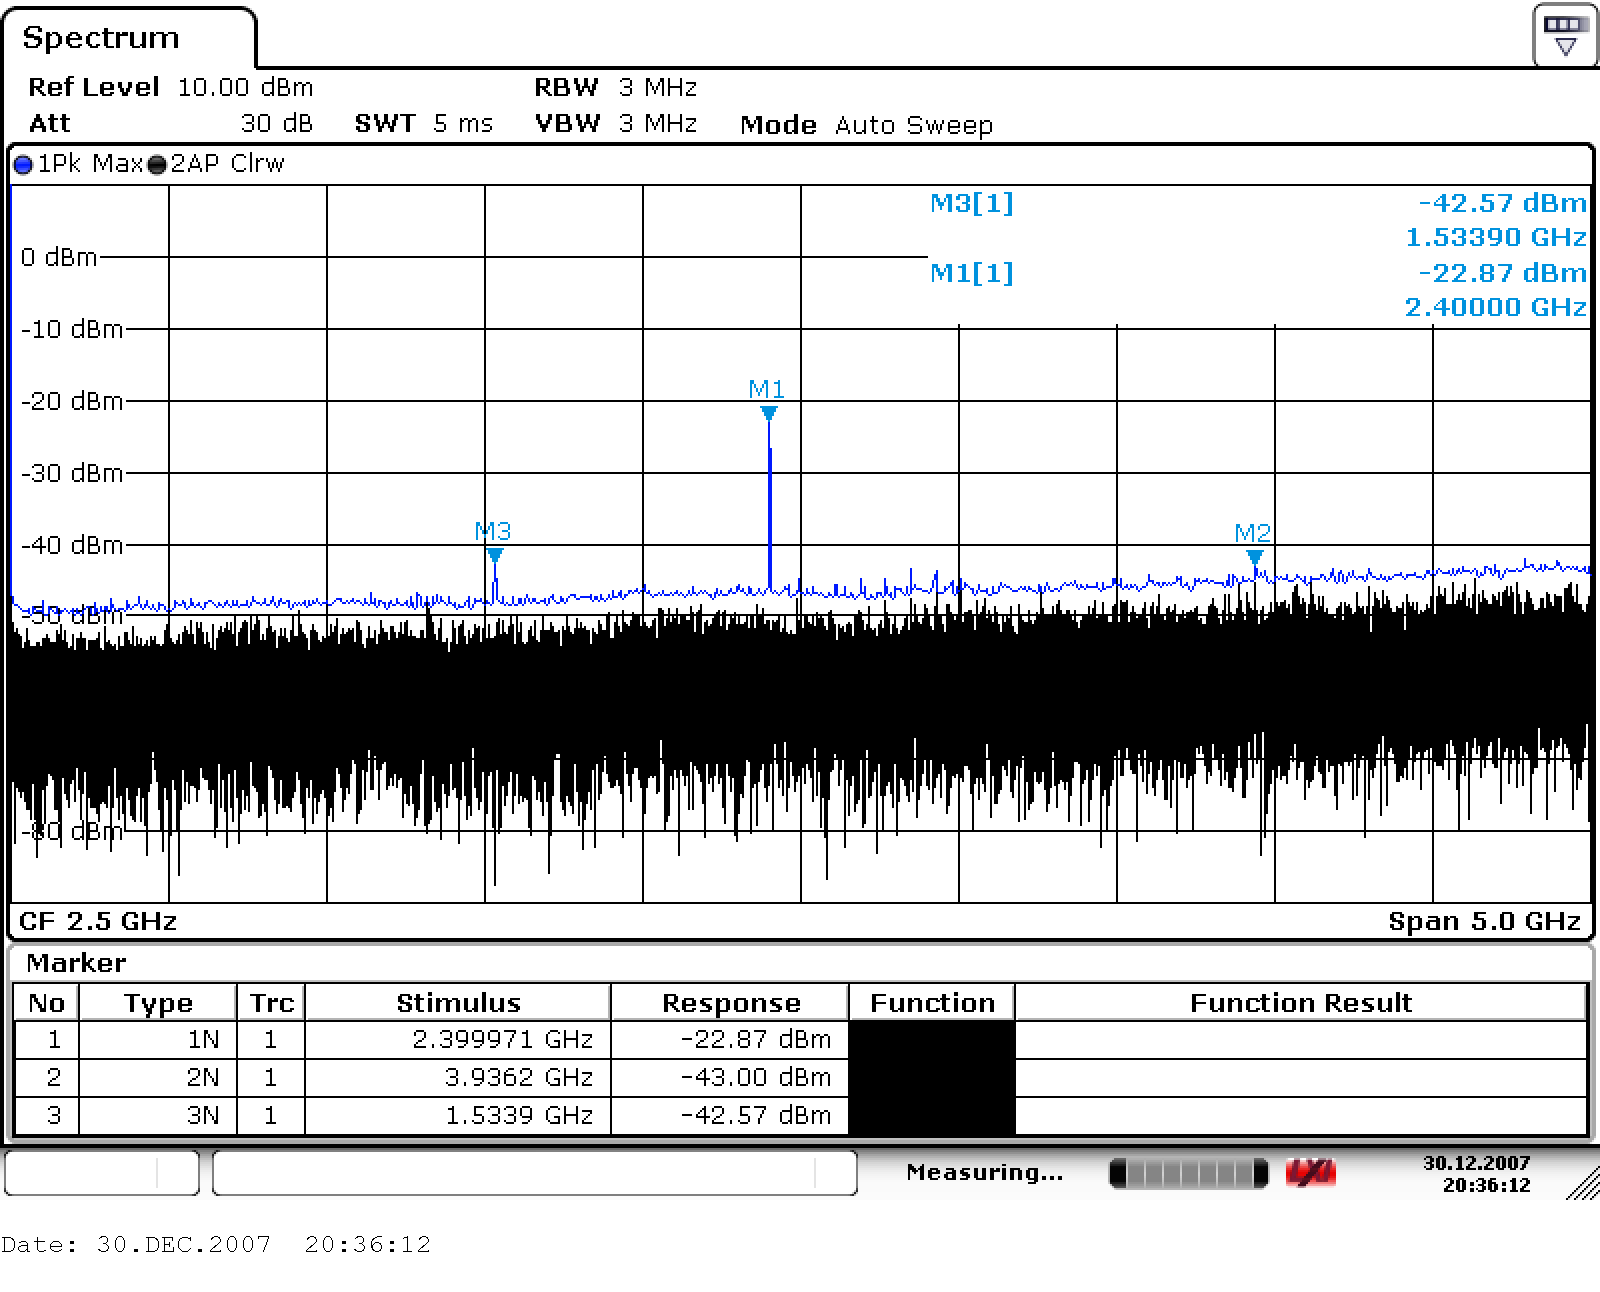
\includegraphics[width=\textwidth,keepaspectratio]{kepek/A_csop_016.PNG}
		\caption{Szűrés után}
		\label{fig:RF_utana}
	\end{subfigure}
	\caption{RF keverés utáni szűrt, illetve szűretlen kimeneti spektrum.}
	\label{fig:RF}
\end{figure}

A teljes összeépített adóláncot, amit a mérés során összeépítettünk a \ref{fig:adolanc}. ábrán láthatjuk.

\begin{figure}[H]
	\centering
	%\includegraphics[width=0.75\textwidth,keepaspectratio]{kepek/?}
	\caption{A teljes adólánc}
	\label{fig:adolanc}
\end{figure}

\section*{Vevőlánc}

% Jancsi, tiéd a pálya



































